\documentclass[%
reprint,
superscriptaddress,
%groupedaddress,
%unsortedaddress,
%runinaddress,
%frontmatterverbose, 
%preprint,
%preprintnumbers,
%nofootinbib,
%nobibnotes,
%bibnotes,
 prl,
 amsmath,
 amssymb,
 aps,
 longbibliography
%pra,
%prb,
%rmp,
%prstab,
%prstper,
%floatfix,
]{revtex4-2}

%\UseRawInputEncoding
%\documentclass[pdflatex,sn-mathphys]{sn-jnl}

\usepackage{cancel}
\usepackage{dcolumn}% Align table columns on decimal point
\usepackage{bm}% bold math
\usepackage[usenames,dvipsnames]{color}
\usepackage{soul}
\usepackage{subcaption}
\usepackage{enumitem}
\usepackage{xspace}
\usepackage{booktabs}
\usepackage{lipsum}
\usepackage[ISO]{diffcoeff}
\usepackage{ragged2e}
\usepackage{mathrsfs}
%\usepackage[capitalise]{cleveref}
\usepackage[normalem]{ulem}
\usepackage{wrapfig}
\usepackage{esvect} %for correct vectors using \vv
\usepackage{titlesec}
\usepackage{titletoc}
\usepackage{chngcntr}
\usepackage{fontawesome5}
\usepackage{mleftright}
\usepackage[nodayofweek]{datetime}
\usepackage{comment}

\usepackage{graphicx}
\usepackage{amsmath}
\usepackage{amsfonts}
\usepackage{array}
\usepackage{siunitx}
\usepackage{bookmark}
\usepackage{natbib,hyperref}
\usepackage{gensymb}
%\usepackage{authblk}
\usepackage{textgreek}
\usepackage{caption}
% Deze hieronder zorgt dat plaatjes binnen section blijven
\usepackage[section]{placeins}
%\usepackage{ccaption}
%\captionsetup[table]{position=below}
%\usepackage[usenames,dvipsnames]{color}
\usepackage{xcolor}
\usepackage{dblfloatfix}
\usepackage{caption}

\renewcommand{\dbltopfraction}{0.9}
\renewcommand{\dblfloatpagefraction}{0.8}


\sisetup{
    exponent-product = \cdot,
    range-phrase = -,
    range-units = single,
    detect-weight = true,
    detect-family = true,
    detect-all = true}

\captionsetup{justification=raggedright,singlelinecheck=false}

%\jyear{2022}
\raggedbottom
\definecolor{firebrick}{HTML}{B22222}

\hypersetup{
    colorlinks=true,       % false: boxed links; true: colored links
    linkcolor=firebrick,          % color of internal linkshttps://www.overleaf.com/project/65dd05895a901323fe62bed3
    citecolor=firebrick,        % color of links to bibliography
    filecolor=firebrick,      % color of file links
    urlcolor=firebrick           % color of external links
}

\definecolor{orcid-green}{RGB} {166, 206, 57}
\newcommand{\MYhref}[3][blue]{\href{#2}{\color{#1}{#3}}}%

\titleclass{\mysection}{straight}[\section]
\titleformat{\mysection}[runin]
  {\itshape}{\thesection}{}{}[.---]
\titlespacing{\mysection}{1em}{1em}{0em}


%\renewcommand{\thesection}{\Alph{section}}
%\titleclass{\myappsection}{straight}[\section]
%\titleformat{\myappsection}[hang]
%  {\bfseries}{\refstepcounter{section}Appendix \thesection}{1em}{}
%\titlespacing{\myappsection}{1em}{1em}{0em}


\newcommand{\red}{\textcolor{red}}
\newcommand{\blue}{\textcolor{blue}}
\newcommand{\THO}[1]{{\textcolor{blue}{{[\bf THO: #1]}}}}
\newcommand{\DU}[1]{{\textcolor{orange}{{[\bf DU: #1]}}}}
\newcommand{\JWL}[1]{{\textcolor{cyan}{{[\bf JWL: #1]}}}}

\newcommand{\kB}{k_\text{B}} %because it should be a text{B} and this is quicker to type

\begin{document}

%These two are usefull for the appendix
\newcommand{\titleinfo}{\boldmath Picometer control of a levitating milligram gravity sensor}
\newcommand{\authorinfo}{Dennis G.~Uitenbroek, Jurriaan Langendorff, and Tjerk H.~Oosterkamp}

\title{\titleinfo}

\author{Dennis G.~Uitenbroek\,\MYhref[orcid-green]{https://orcid.org/0009-0008-3425-6406}{\faOrcid}}
\affiliation{Leiden Institute of Physics, Leiden University, P.O. Box 9504, 2300 RA Leiden, The Netherlands.}

\author{Jurriaan Langendorff\,\MYhref[orcid-green]{https://orcid.org/}{\faOrcid}}
\affiliation{Leiden Institute of Physics, Leiden University, P.O. Box 9504, 2300 RA Leiden, The Netherlands.}

\author{Tjerk H.~Oosterkamp\,\MYhref[orcid-green]{https://orcid.org/0000-0001-6855-5190}{\faOrcid}}
\affiliation{Leiden Institute of Physics, Leiden University, P.O. Box 9504, 2300 RA Leiden, The Netherlands.}



\begin{abstract}
\noindent
Due to their exceptional isolation from the environment, magnetically levitated particles are explored as extremely sensitive mechanical sensors. For future gravity experiments on quantum superpositions, such systems need to be cooled close to their ground state. To demonstrate the combination of state of the art vibration isolation, milligram levitated high Q mechanical resonators and position detection with low noise, we present linear feedback cooling of a magnetically levitated gravity sensor to below 2 picometer amplitude and below 10 millikelvin mode temperature for two translational modes (the x- and y-mode) simultaneously. The sensor is a levitating permanent magnet in a type I superconducting trap, where its six resonance frequencies are measured with a superconducting coil coupled to a DC SQUID.  This signal is measured with a lock-in amplifier and a feedback signal is sent to a piezoelectric actuator, allowing the cooling of resonant modes  at \SI{50.6}{} and \SI{68.0}{Hz} simultaneously. These two translational modes have Q factors of \SI{3.8e6}{} and \SI{5.5e6}{} respectively. The experiment is mounted inside a dry dilution refrigerator where it is vibrationally attenuated with \SIrange{110}{130}{dB} at these frequencies. In this work, we discuss future improvements on the setup which may enable quantum ground state cooling on a magnetically levitated particle, that has previously been shown to be a gravitational sensor.
\end{abstract}
\maketitle

%\section{Te bespreken} 
%\begin{itemize}
%    \item 
%\end{itemize}

\mysection{Introduction}\label{sec:introduction}

%Over massa heel nauwkeurig meten, nog te lezen https://pubs.acs.org/doi/full/10.1021/acs.nanolett.9b00082
\begin{comment}
\DU{Suggestie van Bas: Als ik mijn persoonlijke favoriet mag geven van de onderdelen die al terugkomen in de paper zou ik zeggen dat de stertkste verhaallijn is:
\begin{itemize}
\item quantum experimenten met grote massas zijn belangrijk
\item om een quantum experiment te doen moet je je mode nabij de quantum ground state koelen
\item GS cooling kan met clamped resonators 
\item maar ivm clamping lsoees  moeten we levitatie dien  (wat niet in je tekst staat, maar volgens mij ook cruciaal is op termijn: dynamische controle over de potentiaal. Misschien heb je dat expres weggelaten ivm het feit dat je dat bij jullie trap juist niet hebt.)
\item optische systemen kunnen GS koelen, maar hebben te weinig massa en werken bij hoge frequencie
\item Magnetishe levitatie is belangrijk want a) grotere massas mogenlijk en b) geen inernal heating door de trapping laser
\item MAAAR a) dan gaan wel zeker je frequencites omlaag en word vibratie isilatie veel lastiger. b) dan wordt detectie ook moeilijker
\\
\item HERE: state of-the art vibratie isolaie in combinatie met zeer zwaar geleviteerd deeltje met hoge Q factor en low-noise readout. Om te benchmarken hoe goed dit allemaal al is doe je mode-cooling.  Misschien ook nadruk leggen dat het allemaal tegelijk goed moet zijn.
\end{itemize}}
\end{comment}
Large mass quantum experiments are the key ingredient in closing the gap between microscopic quantum systems and macroscopic general relativity. By pushing the quantum effects to larger and heavier scales, an experiment combining these two theories could be enabled. Observing quantum mechanical effects in a mechanical system requires a crucial first step: cooling a particle close to the mechanical quantum ground state. This has been a goal within the physics community on various platforms using different cooling methods. Additionally, one would like to achieve this quantum regime in a mass regime where gravity becomes relevant.

In early work, micromechanical membranes were shown to be cooled to the quantum ground state~\cite{Connell2010, Teufel2011, Chan2011, Safavi2012, Jockel2015}. These type of systems will inevitably suffer from clamping losses, due to the suspended nature of these experiments.
% More recently a cat state in a similar system is shown, with an effective mass up to \SI{16}{ug} (nog checken of niet al meer) [ref Bild et al. misschien nog meer].

In an effort to avoid clamping losses, levitated systems can be studied. Trapped ions were the first to be cooled to the mechanical groundstate, using laser sideband cooling~\cite{Diedrich1989, Monroe1995, Leibfried2003}. Although impressive results are accomplished in this field, these type of experiments are limited to very few atoms in scale.

In optical levitation, groundstate cooling has been achieved~\cite{Delic2020, Tebbenjohanns2021, Magrini2021, piotrowski2023} since a couple of years. These experiments are performed at relatively high frequencies (\SI{10}{k\hertz} - \SI{1}{M\hertz}) compared to magnetic levitation. At these frequencies mechanical vibrations are less present and can be readily attenuated. This is a very promising platform for pushing the limits of quantum mechanical effects. However, these particles have a size around \SI{100}{nm} and a mass in the order of femtograms. This is already a large step in macroscopicity compared to ions, but still far from a macroscopic particle that would generate a measurable amount of gravity.

A different levitation platform, magnetic levitation, makes use of magnetic forces. This platform is not limited in mass due to the magnetic forces and there is no internal heating of the particle as in the above-mentioned levitation systems. With the larger mass the frequencies will decrease (compared to optical levitation). At these lower frequencies dampening the mechanical vibrations is more challenging.

Different types of magnetic levitation exist, we will only discuss superconducting levitation here, superconducting levitation can be divided in active~\cite{Bob, Gutierrez2020, Gutierrez2022, Hofer2023, Gutierrez2023, Schmidt2024, Paradkar2025, Hansen2026} and passive systems~\cite{Timberlake2019, Vinante2020, Vinante2022, Timberlake2024}. Active systems send a current through coils that levitate a piece of superconducting material by using the perfect diamagnetic properties of the superconductor. The passive systems use the same perfect diamagnetic property due to the Meissner effect and let the superconductor expel the magnetic field, coming from a permanent magnet. Both mechanisms are, in principle, scalable to sizes greater than \SI{1}{mm}. The advantage of a passive system is the absence of noise sources from the active components, e.g. the current noise in the coils.

Passive magnetic levitation with a submillimeter particle of \SI{0.43}{mg} has already been demonstrated in a gravitational experiment~\cite{Gravity}. In this letter, a version of this setup with state-of-the-art vibration isolation, a massive levitated particle with high Q factors, and low noise readout are all together combined to reduce the motion of the particle to below two picometer of RMS amplitude. This achieved motion is a benchmark for the performance of the system, this can only be achieved if all necessary experimental conditions are fulfilled simultaneously. Performing ground state cooling on these type of systems is possible in theory, but experimentally very challenging. The zero point motion scales with $\sim 1/\sqrt{m \omega}$. In magnetic levitation the relatively large masses in combination with low frequencies result in a small zero point motion, \SI{0.7}{fm} for the setup used here.

%In this letter, a version of this setup with larger detection sensitivity is used to measure the mode temperature of two of the six degrees of freedom. These two modes are cooled by means of applying linear feedback to a piezoelectric element attached to the superconducting trap. Performing ground state cooling on these type of systems is in theory possible, but experimentally very challenging. The zero point motion scales with $\sim 1/\sqrt{m \omega}$. In magnetic levitation the relatively large masses in combination with low frequencies result in a small zero point motion, \SI{0.7}{fm} for the setup used here. Sufficient damping of mechanical noise at the resonance frequencies (\SIrange{15}{200}{Hz}) is required in combination with the cryogenic environment. The experimental setup makes use of several vibration isolation systems, both passive and active. Despite these efforts, mechanical noise is still affecting the experiment, mainly through upconversion of vibrations.

In this experiment a phonon number in the order of \SI{e6}{} is reached. The theoretical minimum phonon limit with current detection and force noise is in the order of \SI{e5}{} phonons. With improvements on vibration isolation, Q factors, detection coupling and SQUID noise, we think it would be possible to cool this system to the ground state. 
Since this setup has already been used for gravitational measurements~\cite{Gravity}, combining this system with the feedback cooling presented in this paper, this experiment demonstrates to be a promising platform towards combining both gravitational interaction and quantum mechanical effects in a single experiment.

%However, this experimental platform is a promising route to cool macroscopic particles to the quantum ground state.
    

\mysection{Experimental setup}\label{sec:setup}
%We demonstrate linear feedback cooling of two translational modes simultaneously. 
The experiment consists of a permanent magnet levitating in a superconducting trap by Meissner repulsion. The motion of the magnet is measured using a Superconducting QUantum Interference Device (SQUID) measured by a lock-in amplifier. The lock-in then calculates a feedback signal and sends this to a piezoelectric actuator, schematically shown in Fig.~\ref{fig:setup}a.

%A piezoelectric actuator is used to cool translational modes by means of linear feedback. 

%The experiment is performed at the bottom of an extensive vibration isolation system inside a dry dilution refrigerator, and is schematically shown in Fig.~\ref{fig:setup}a. Cooling to the quantum ground state with the same technique is possible, with additional vibration isolation particularly for the lower frequencies (resonances of the vibration isolation system), and improved detection coupling with the use of a quantum limited SQUID.

The permanent levitating magnet is composed of three \SI{0.25}{mm} by \SI{0.25}{mm} by \SI{0.25}{mm} cubic neodymium iron boron parylene coated magnets stacked and glued together, using Stycast. A glass sphere with a diameter of \SI{0.20}{mm} is attached to this stack of magnets, again using Stycast, see Fig.~\ref{fig:setup}b. The glass sphere is placed off center to break symmetry. Typical permanent remnant magnetisation of these magnets is \SI{1.4}{T}, although it is believed that at low temperatures this is reduced by \SIrange{20}{25}{\%}~\cite{NdFeB_SmCo_Technotes}. The estimated mass of this composed magnet and glass sphere is \SI{0.35}{mg}.

The magnet levitates in a type I superconducting trap made of tantalum, shown in Fig.~\ref{fig:setup}c. This trap has an elliptical shape, \SI{3.0}{mm} by \SI{4.0}{mm} as the minor and major axes. The pick-up coil is placed at a height of \SI{4.0}{mm} from the bottom of the trap. The calculated levitation height of the magnet is \SI{1.96}{mm}~\cite{Vinante2020}. The pick-up coil is able to detect the motion of the magnet, via the induced current in the pick-up coil. The pick-up coil is part of the detection scheme consisting of the pick-up coil, the calibration transformer, and the SQUID input coil. The calibration transformer is used to calibrate the coupling between the detection circuit and the six different degrees of motion of the magnet. A schematic overview of the detection can be seen in Fig.~\ref{fig:setup}a.
%levitation height: https://www.wolframalpha.com/input?i=%28%283*mu_0*%283*0.25mm*0.25mm*0.25mm*1.4T%2Fmu_0%29%5E2+%29+%2F+%2864*pi*0.354e-6+kg*9.81m%2Fs%5E2%29%29%5E%281%2F4%29

\begin{figure}[t!]
    \centering
    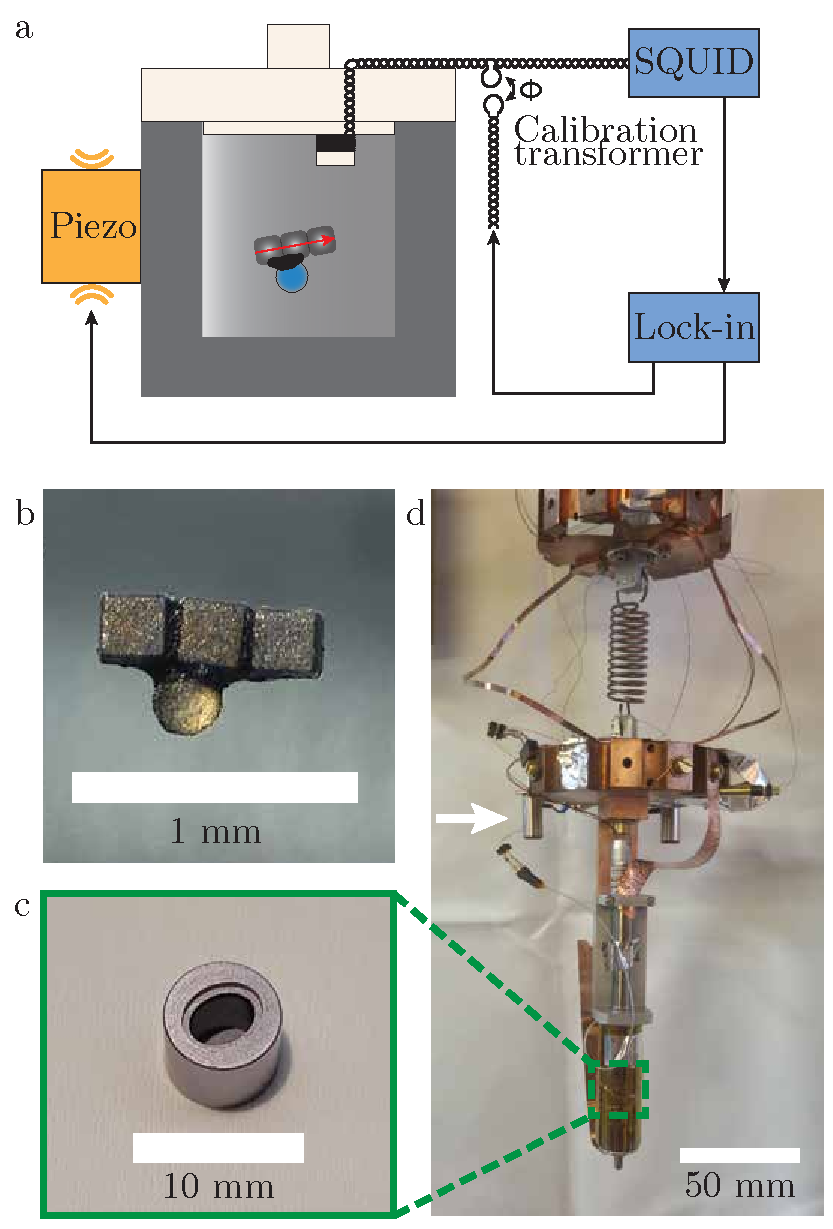
\includegraphics[width=\columnwidth]{Figures/Figure_setup_new_V2.pdf}
    \caption{Overview of the experimental setup. (a) A schematic outline of the setup, the levitating permanent magnet is shown inside the superconducting trap. A pick-up coil attached to the lid of the trap picks up the varying flux of the moving levitated magnet and is detected using a two stage SQUID amplifier. We feedback cool the magnets motion by applying a phase shifted tone shaking the trap housing through a piezo and lock-in amplifier. (b) A close-up of the permanent magnet used in the experiment. It is composed of three \SI{0.25}{mm} cubic neodymium iron boron parylene coated magnets stacked and glued together. A glass sphere with a diameter of \SI{0.20}{mm} is attached to this stack of magnets using Stycast, to break rotational symmetries. (c) Picture of the elliptically shaped superconducting trap, made from tantalum. (d) Closeup of the bottom part of the multi-stage mass spring system where the magnet, trap and piezo are located. The trap is located inside the magnetic shielding, indicated with the green dashed lines. The piezo is attached to the lowest copper mass and indicated with a white arrow.}
    \label{fig:setup}
\end{figure}

Vibrational noise is suppressed by a multistage mass spring system both in the vertical and lateral directions. The lowest two masses and one of the springs can be seen in Fig.~\ref{fig:setup}d. The experiment is rigidly attached to a copper mass, which is suspended from two other copper masses with springs in between. The lowest resonance frequencies are at \SI{0.6}{Hz} and \SI{1}{Hz} along the lateral and vertical directions, respectively. These three stages are thermalised to the millikelvin stage inside a dry dilution 

%\DU{De opmaak hier is vrij lastig, moet helaas met de hand}
\clearpage
\begin{widetext}
\begin{figure}[t]
    %\centering
    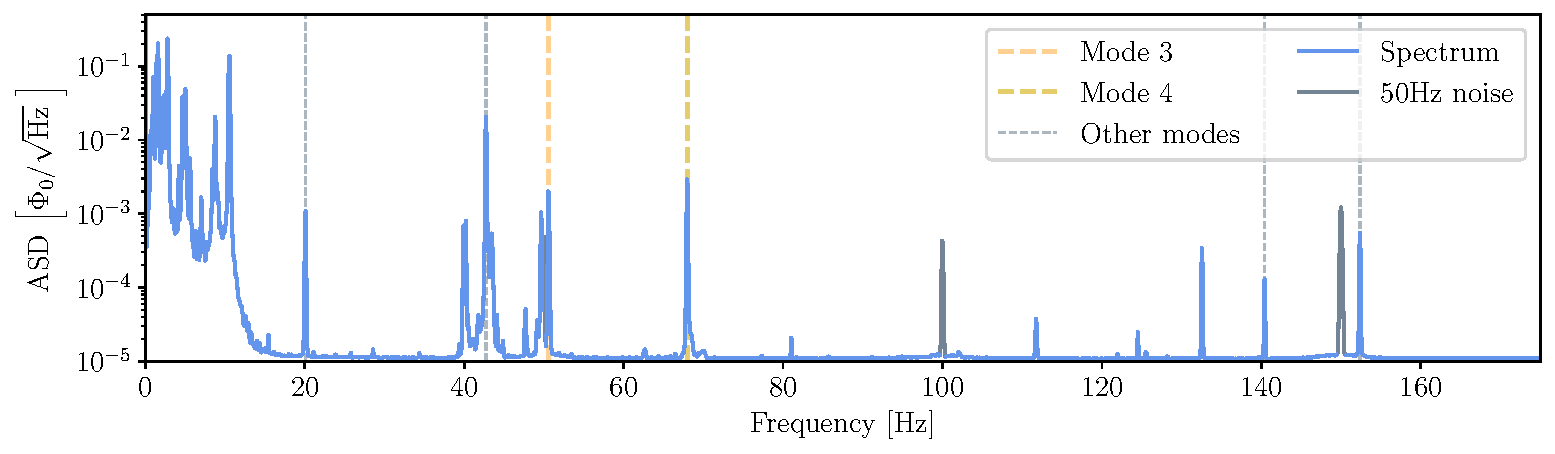
\includegraphics[width=\textwidth]{Figures/paper_figure_spectrum_20260307_during_the_day.pdf}
    \begin{minipage}{\textwidth}
    \caption{Typical amplitude spectral density (ASD) of the levitated magnet, the resonant modes of the magnet are indicated with the dotted lines. In this figure the \SI{50}{Hz} European electrical noise is grayed out.}
    \label{fig:spectrum} \end{minipage}
\end{figure}
\end{widetext}

\noindent
refrigerator. In the current configuration, the mass spring system is suspended from the still plate in order to utilize the additional available vertical length. For further attenuation, the still plate is suspended by springs from the \SI{3}{K} plate. 

The cryostat as a whole is rigidly attached to a 25-metric ton concrete block located in the cellar of the building, placed on pneumatic dampers to limit vibrations. The pulse tube and circulation pumps are rigidly attached to the building via a second frame. We typically measure between \SI{110}{} and \SI{130}{dB} attenuation in energy at a frequency range of \SIrange{50}{70}{Hz}, for this system. This is consistent with a finite element simulation, which show between \SI{160}{} to \SI{180}{dB} under idealized conditions, see supplementary material Fig.~\ref{fig:spectrum_attenuation}. 

%\red{We typically measure 80 dB attenuation in a frequency range of \SIrange{15}{80}{Hz}, for this system.\red{eventueel nog iets zeggen (apart) over 80-180Hz)} This is in agreement with a finite element model.}  
%The experiment is rigidly attached to a copper mass, which is hanging from two other copper masses, with a \textcolor{cyan}{lowest resonance frequency at \SI{10.67}{Hz}.} \DU{@Jurriaan?} These three stages are all thermalised to the millikelvin stage inside the dry dilution refrigerator. The mass spring system, however, is hanging from the still plate to use the extra length. For further attenuation, the still plate is suspended by springs from the \SI{3}{K} stage. The cryostat as a whole is rigidly attached to a 25-metric ton concrete block located in the cellar of the building, placed on pneumatic dampers to limit vibrations. The pulse tube and circulation pumps are rigidly attached to the building via a second frame.

%A piezoelectric actuator is rigidly attached to the mass to which the superconducting trap is attached, to enable a feedback force on the particle. The motion of the particle is measured using the pick-up coil, via a DC SQUID. 

The SQUID signal is processed at different frequencies simultaneously by a lock-in amplifier, which then provides a linear feedback signal which is sent to the piezo with the proper phase shift, to decrease the amplitude of the motion of the particle. The feedback gain can be altered to vary the effective damping.

Once the magnet is levitating, many clear peaks in the spectrum are visible, shown in Fig.~\ref{fig:spectrum}. Six peaks correspond to six degrees of freedom of the levitating magnet, three translational and three rotational. The lowest frequency and the highest two frequencies are believed to be rotational modes, mode 2 is believed to be the translational z-mode and mode 3 and 4 are believed to be the y-, and x-translational modes respectively, see supplementary material~\ref{sec:mode identification} for details on the mode identification. Based on coupling and sensitivity, mode 3 and mode 4 were chosen to cool using linear feedback with the piezo.

The motion of the particle is calibrated using the calibration transformer. A current is sent through this coil, the energy sent into the superconducting detection circuit and the energy gain in the motion of the particle are both measured. This together with known properties of the circuit and the magnet, provides the absolute calibration of the motion, in units $\SI{}{V/m}$. Further details can be found in supplementary material~\ref{sec:calibration}. Note that other peaks in the spectrum are due to magnetic or mechanical noise, but these cannot be excited with the calibration coil.

The response of the levitating magnet to the linear feedback signal can be calculated from the following equation of motion
\begin{equation}
    m \ddot{x}(t) + \gamma_\text{0} \dot{x}(t) + kx(t) = F_\text{tot}(t) = F_\text{th}(t) + F_\text{FB}(t).
    %F_{th} - g \gamma \left( \dot{x} + \dot{x}_n \right).
\end{equation}

In this equation $m$ is the mass of the magnet, $x(t)$ is the position, $\gamma_0$ is the mechanical damping in the system, with units $\SI{}{N/(m/sec)} = \SI{}{kg/sec}$. Furthermore, $k$ is the spring constant of the mode, $F_\text{tot}$ is the total force acting on the particle, $F_\text{th}$ is the random thermal force and $F_\text{FB}$ is the feedback force. This feedback force provides a feedback damping ($\Gamma_\text{FB}$) for which the proportional gain can be set, this is an additional damping to the damping in the system ($\Gamma_\text{0}=\gamma_0/m$). When the phase of the feedback force is chosen correctly such that the feedback force is proportional to the velocity of the particle, this equation of motion has a corresponding power spectral density (PSD) with units $\SI{}{m^2/Hz}$

\begin{equation}
    S_{x}(\omega) = \frac{4 \kB T \Gamma_\text{0}}{m} \frac{1}{\left( \omega_0^2 - \omega^2 \right)^2 + \omega^2 \left(\Gamma_\text{0} + \Gamma_\text{FB} \right)^2}.
\end{equation}

For center of mass modes the thermal force noise is given by $S_F = 4 \kB T m \omega_0 / Q$ for rotational modes the torque noise equals $S_\tau = 4 \kB T I \omega_0 / Q$. Here, $\kB$ is the Boltzmann constant, $T$ is the effective temperature formed by the thermodynamic temperature and vibrations at the resonance frequencies, $m$ is the mass, $\omega_0$ is the resonance frequency, $Q$ is the quality factor and $I$ is the moment of inertia. 

This power spectral density can also be expressed as an amplitude spectral density (ASD) in units of $\SI{}{m/\sqrt{Hz}}$ by taking the square root. Because the quality factor is very high, it is sufficient to integrate over a bandwidth ($\text{BW}$) $\left[ f_0-3f_0/Q, f_0+3f_0/Q \right]$ to get 99 percent of the energy. Integrating over this bandwidth, the amplitude ($A_\text{RMS}$) and energy in the mode are calculated. Next, using the equipartition theorem the mode temperature ($T_\text{mode}$) is determined

\begin{align}
    T_\text{mode} = \frac{k}{\kB} \int\displaylimits_\text{BW} S_{x}(\omega) d\omega .
\end{align}

%\DU{Bas had hier een suggestie om een tussenstap te maken van $E_\text{mode}$ is integraal, $A_\text{RMS}$ is E/k en dan $T_\text{mode} = k / \kB E_\text{mode}$. Vind ik zelf omslachtig en niet echt nodig. Wat vinden jullie?}



\begin{comment}
\red{-------Dennis zou dit weglaten ------------}\\
We have $Q = \omega_0 / \Gamma$ \red{misschien nog onderscheid maken met deze en $Q= \pi f \tau$, volgens het blad van Julian.}

\red{Now Hendrik ends up in}
\begin{align}
    T_\text{mode} = T \frac{\Gamma_0}{\Gamma_0 + \Gamma_\text{FB}}
\end{align}

\DU{Waarom doet men dit? THO: Ik denk dat je $g=G_FB/G_0$ kunt definieren en dan is het $T=T*1/(1+g)$ of zo? Je kan toch zeggen dat het de integraal is over $S_x$. Is dat omdat anderen de conversie naar meters (nog) niet kunnen maken op dit punt? THO: eens}\\
\red{-----------------}\\


\DU{Willen we een appendix maken voor de calibratie, of verwijzen we naar die van de gravity paper? THO: zie boven}



\red{--------below here is Martins method------------} \\
The fit values from fig. are used to calculate the final mode temperature, using:
\begin{equation}
    T_\text{mode} = \frac{T}{1+g} + \frac{k \omega_0}{4 \kB Q_0} \left( \frac{g^2}{1+g} \right) S_{x_n}.
\end{equation}

At the maximal gain this corresponds to a mode temperature of \red{\SI{0}{mK}}. 
\end{comment}
\mysection{Results}\label{sec:results}
The described method has been applied to two translational modes simultaneously. The applied feedback signal is a phase shifted version of the measured signal, with a variable gain. The use of the lock-in amplifier ensures that we send a narrow band version of the measured signal, which is difficult with analogue band pass filters. The measured lock-in signal is Fourier transformed using the Welch method, to average over the measurement time. Finally, the bandpass filter of the lock-in is compensated numerically.

The results for mode 3 and mode 4 are plotted in separate figures. In the legend, the values of the achieved mode temperatures with corresponding RMS amplitude and proportional gain are given. Increasing the proportional gain results in lowering the peak, leading to an effective broadening of the peak, as expected. Same colors in the legends of Fig.~\ref{fig:cooling3} and Fig.~\ref{fig:cooling4} correspond to the same moment in time. 

Mode 3 has a resonance frequency of \SI{50.59}{Hz} and a Q factor of \SI{3.8e6}{}. The lowest observed mode temperature for mode 3 is \SI{7.1}{mK}, obtained using a gain of \SI{930}{} and has a corresponding RMS amplitude of \SI{1.6}{pm}. %, see Fig.~\ref{fig:cooling3}.

\begin{figure}[h!]
    \centering
    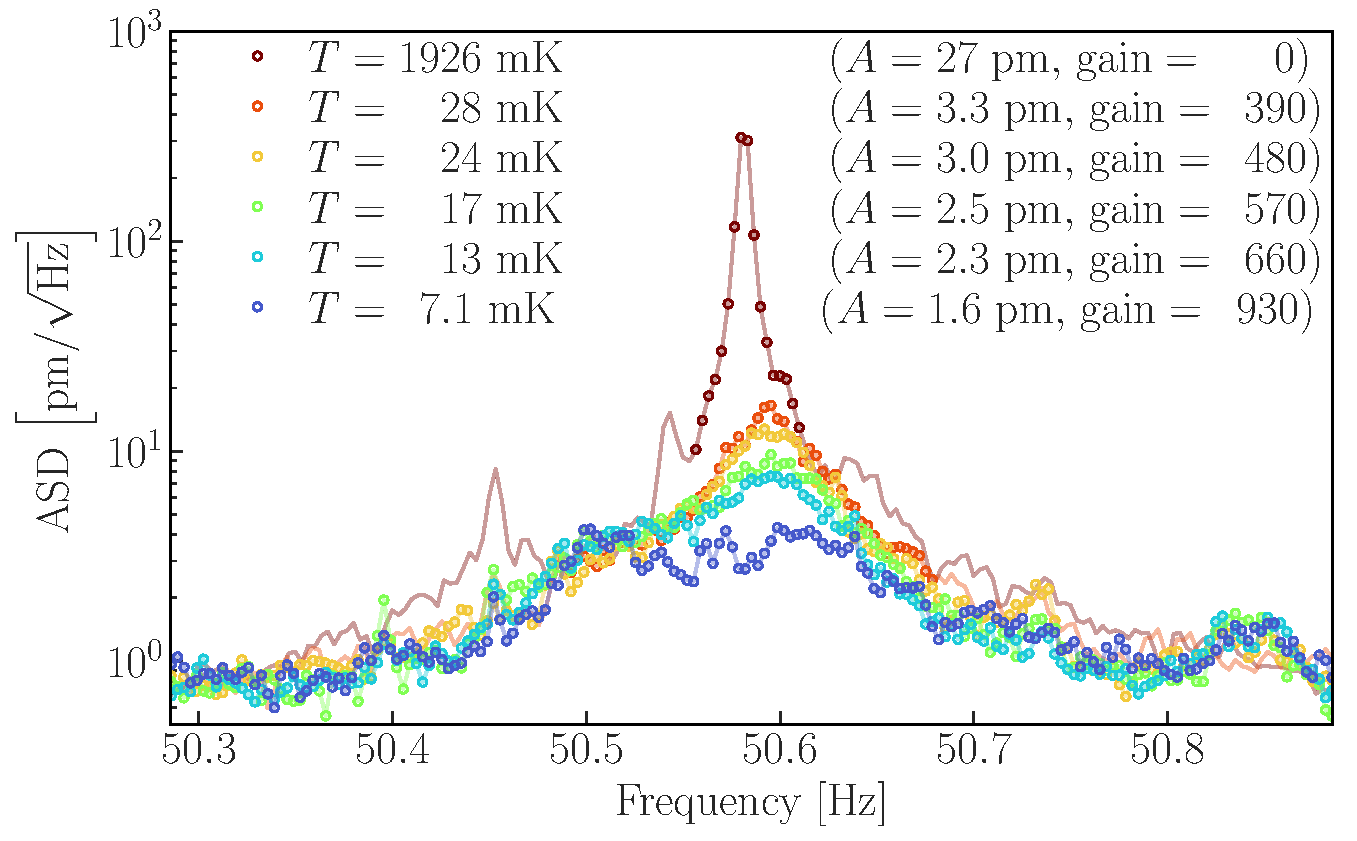
\includegraphics[width=\columnwidth]{Figures/paper_figure_mode_3.pdf}
    \caption{The linear feedback cooling on mode 3 is plotted. The different colored lines represent spectra taken with different linear gains. The legend shows the achieved mode temperatures with corresponding RMS amplitude and proportional gain values. Equal colors in this plot and in Fig.~\ref{fig:cooling4} indicate measurements are taken simultaneously.}
    \label{fig:cooling3}
\end{figure}

%\DU{Bas had bedacht om in deze twee figuren weer mode en RMS als subscript bij te zetten. Als we zouden wisselen naar de gamma FB notatie past dat wellicht wel. Louisa merkt op dat de gain nu geen betekenis heeft. Dat we beter naar dB of naar Gamma FB kunnen wisselen. Ik vind dat ze wel een punt heeft alleen dat we dat nu niet makkelijk kunnen doen toch?}\\
%\DU{Een andere suggestie van Bas is om het hier als $\sqrt{S_x} [pm/\sqrt{Hz}]$ te doen en in Fig. 2 wel als PSD. Wat vinden jullie? Ik heb zelf geen mega sterke mening los van dat ik dit even duidelijk vind als het andere}

Mode 4 has a resonance frequency of \SI{67.98}{Hz} and a Q factor of \SI{5.5e6}{}. The same cooling mechanism is applied to mode 4, in this case the lowest observed mode temperature is \SI{6.6}{mK} simultaneously with the \SI{7.1}{mK} of mode 3. Here, a gain of \SI{1500}{} is used and a corresponding RMS amplitude of \SI{1.2}{pm} is measured.

Both plots show lines and dots, the lines represent the measured data. The part of the data that falls within the mentioned bandwidth ($\text{BW}$) of $\left[ f_0-3f_0/Q, f_0+3f_0/Q \right]$ is visualised with the dots in both Fig.~\ref{fig:cooling3} and Fig.~\ref{fig:cooling4}. The shown RMS amplitude and mode temperature are therefore based on the cumulative sum of these dots. 

\begin{figure}[h]
    \centering
    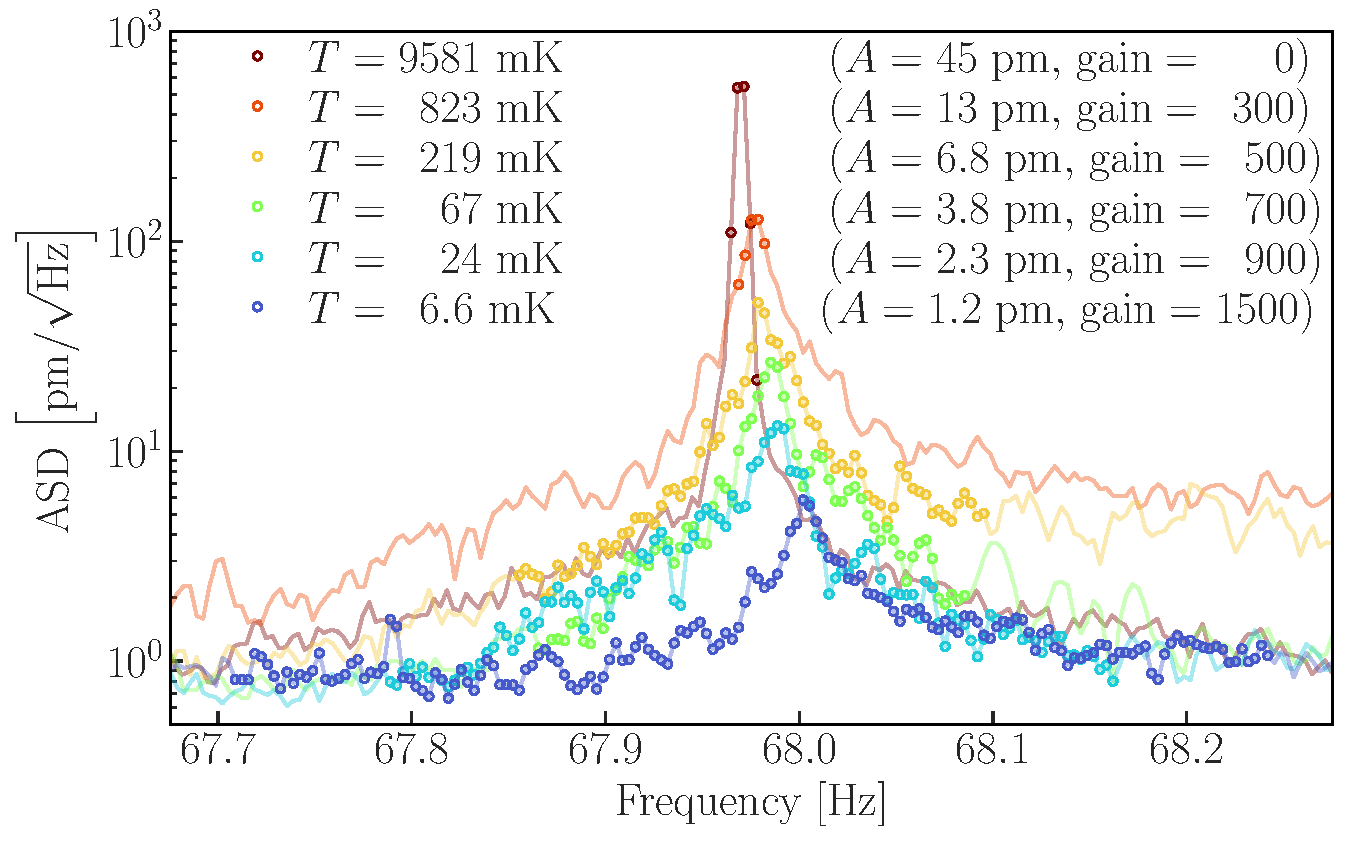
\includegraphics[width=\columnwidth]{Figures/paper_figure_mode_4.pdf}
    \caption{Similar to Fig.~\ref{fig:cooling3}, the linear feedback cooling on mode 4 is plotted. The different colored lines represent spectra taken with different linear gains. The legend shows the achieved mode temperatures with corresponding RMS amplitude and proportional gain values. Equal colors in this plot and in Fig.~\ref{fig:cooling3} indicate measurements are taken simultaneously.}
    \label{fig:cooling4}
\end{figure}

These results are achieved while not only doing active feedback on mode 3 and 4, but also on some of the mass spring system modes and on mode 2 with a second piezo. Active feedback is applied on these frequencies continuously to ensure a relatively quiet environment for the linear feedback on mode 3 and 4. During these measurements upconversion of noise peaks surrounding the resonance peaks is visible in the spectrum, see supplementary material~\ref{sec:mode mixing} for further details.

Mode temperature can be converted to a phonon number ($N_\text{ph}$) via:

\begin{equation}
    N_\text{ph} = \frac{k_B T_\text{mode}}{\hbar \omega_0}.
\end{equation}

In the case of mode 3 the lowest mode temperature corresponds to a value of $N_\text{ph, 3} = \SI{2.9e6}{}$ and for mode 4 a value of $N_\text{ph, 4} = \SI{2.0e6}{}$.


\mysection{Conclusion}\label{sec:conclusion}
In conlusion, we have performed linear feedback cooling to a magnetically levitated particle of submillimeter scale in a superconducting trap. Two different translational modes (the y- and x-mode) have simultaneously reached \SI{7.1}{mk} and \SI{6.6}{mK}. This is performed in a dry dilution refrigerator, with extensive vibration isolation. The mass of the levitated particle is \SI{0.38}{mg} and the feedback cooled phonon number is \SI{2.9e6}{} and \SI{2.0e6}{}, for mode 3 and 4 respectively.

Currently, we are limited by detection sensitivity and upconversion of resonances of the vibration isolation system below \SI{10}{Hz}. Improvements on the achieved mode temperatures in this experiment can be achieved with lower starting temperatures and/or lower force noise (i.e.  better vibration isolation), higher Q factors (which will also require an even better vibration isolation) and lower detection noise (which can be achieved by a larger coupling, i.e. placing the pick-up coil closer to the magnet). 

We can calculate the minimal achievable mode temperature and the corresponding phonon number of the current setup, due to force and detection noise:
\begin{comment}
\begin{equation}
    T_\text{min} = \sqrt{\frac{\omega_0}{2 \kB} \frac{k}{Q_0} S_{x_d}}
\end{equation}
\end{comment}
\begin{equation}
    T_\text{min} = \frac{\omega_0}{2 \kB} \sqrt{ S_F S_{x_\text{det}}}
\end{equation}

Reading from both Fig.~\ref{fig:cooling3} and Fig.~\ref{fig:cooling4} a position noise of $\SI{1}{pm/\sqrt{Hz}}$, and using the uncooled ($\text{gain} =0$) mode temperatures for the force noise, for mode 3 this results in $T_\text{min, 3} = \SI{0.65}{mK}$ and $N_\text{ph, min, 3} = \SI{2.7e5}{}$, and for mode 4 this results in $T_\text{min, 4} = \SI{1.9}{mK}$ and $N_\text{ph, min, 4} = \SI{5.7e5}{}$ as the minimal achievable values with the current setup. 
% mode 3 T: https://www.wolframalpha.com/input?i=%282*pi*50.59Hz%29%2F%282*boltzmann+constant%29+*+sqrt%284+boltzmann+constant*1926mK+*0.35mg*2*pi*50.59Hz%2F3.77e6*+%281pm%2Fsqrt%28Hz%29%29%5E2%29
%mode 3 phonons: https://www.wolframalpha.com/input?i=1%2F%282*hbar%29+*sqrt%284+boltzmann+constant*1926mK+*0.35mg*2*pi*50.59Hz%2F3.77e6*+%281pm%2Fsqrt%28Hz%29%29%5E2%29
%mode 4 T: https://www.wolframalpha.com/input?i=%282*pi*67.98Hz%29%2F%282*boltzmann+constant%29+*+sqrt%284+boltzmann+constant*9581mK+*0.35mg*2*pi*67.98Hz%2F5.45e6*+%281pm%2Fsqrt%28Hz%29%29%5E2%29
%mode 4 phonons: https://www.wolframalpha.com/input?i=1%2F%282*hbar%29+*sqrt%284+boltzmann+constant*9581mK+*0.35mg*2*pi*67.98Hz%2F5.45e6*+%281pm%2Fsqrt%28Hz%29%29%5E2%29

Keeping the current detection sensitivity, but improving the vibration isolation such that upconversion is no longer an issue and the force noise is determined by the thermodynamic temperature of the environment (\SI{20}{mK}), the phonon numbers would fall to \SI{2.7e4}{} for mode 3 and \SI{2.6e4}{} for mode 4. The current magnet, at a frequency of \SI{50}{Hz}, has a zero point motion of \SI{0.7}{fm}, this corresponds to a mode temperature of \SI{2.4}{nK}.
% mode 3: https://www.wolframalpha.com/input?i=1%2F%282*hbar%29+*sqrt%284+boltzmann+constant*20mK+*0.35mg*2*pi*50.59Hz%2F3.77e6*+%281pm%2Fsqrt%28Hz%29%29%5E2%29
% mode 4: https://www.wolframalpha.com/input?i=1%2F%282*hbar%29+*sqrt%284+boltzmann+constant*20mK+*0.35mg*2*pi*67.98Hz%2F5.45e6*+%281pm%2Fsqrt%28Hz%29%29%5E2%29
% x_zpm: https://www.wolframalpha.com/input?i=sqrt%28hbar+%2F+%282+*+0.35+mg+*+2+*+pi+*+50Hz%29%29
% T_zpm: https://www.wolframalpha.com/input?i=hbar+*+2+*pi+*+50+Hz+%2F+boltzmann+constant

In a more extreme case where the setup would be pushed towards its limits, with a thermodynamic temperature of \SI{2}{mK}~\cite{Loek, DeWitVibIso}, a 10 times higher Q factor, a detection sensitivity of $\SI{0.01}{pm/\sqrt{Hz}}$, we would be able to cool mode 3 to \SI{27}{} phonons and mode 4 to \SI{26}{} phonons.
% mode 3: https://www.wolframalpha.com/input?i=1%2F%282*hbar%29+*sqrt%284+boltzmann+constant*2mK+*0.35mg*2*pi*50.59Hz%2F3.77e7*+%280.01pm%2Fsqrt%28Hz%29%29%5E2%29
% mode 4: https://www.wolframalpha.com/input?i=1%2F%282*hbar%29+*sqrt%284+boltzmann+constant*2mK+*0.35mg*2*pi*67.98Hz%2F5.45e7*+%280.01pm%2Fsqrt%28Hz%29%29%5E2%29

%When increasing the measurement coupling
Further improving the experiment and lowering the phonon amount towards the ground state, the back action noise from the SQUID will dominate over the thermal noise of the experiment, at some measurement coupling~\cite{ULDM}. This calls upon improving the SQUID noise to the quantum limit, since the SQUID we use has an energy resolution of approximately 10.000 times $\hbar$~\cite{ULDM, Ahrens2025, Vinante2021}.

Combining all these improvements, cooling and detection of the levitated particle in the quantum ground state should become possible.

% Furthermore, if the current levitated system is seen as a quantum system, the coherence time can be calculated. During the experiment the bath temperature (temperature of the trap and its surroundings) is typically \SI{20}{mK}. At a resonance frequency of \SI{50}{Hz} this corresponds to a bath phonon occupation of \SI{4.2e8}{}. At this frequency, the ringdown time is \SI{2.4e4}{s}, and the coherence time ($\tau_\text{coh}$) of the system would be $\tau_\text{coh} = \tau_\text{ringdown}/N_\text{ph} = \SI{58}{us}$. \DU{hier nog die andere twee getallen bijzetten}

%\DU{@Tjerk, je had het over 1K is equivalent met 20GHz. Ik kom daar op uit als je neemt $\kB T = hf$. Ik zou zelf denken dat je $1/2 \kB T= hf$ moet nemen.} Tjerk: je hebt twee vrijheidsgraden positie 1/2 kx^2 en snelheid 1/2mv^2. Die hebben allebei 1/2 kBT, dacht ik. N_phonon = k_BT/hf, dacht ik.


\begin{comment}
\vspace{2cm}
To do:
\begin{itemize}
%    \item nadruk leggen op dat het phonon nummer wel hoog is maar dat dit systeem al gebruikt is voor zwaartekracht
%    \item ergens quantum limited squid en betere vib iso (upconversion) noemen. Dan zien we 1fm meten wel zitten
%\item  upconversion noemen in results. Zie hieronder?
%\item DU twijfelt uit zijn hoofd hoe we nu de koeling uitleggen, volgens mij noemen we de welch method e.d. nog nergens
\item
\end{itemize}


    x_\text{zpm} = \sqrt{\frac{\hbar}{2 m \omega_0}}

\DU{met een 10 keer hogere koppeling, dus 100 keer hogere m/V, en een quantum limited squid (10.000). Dan nog start T 100x lager, dan ben je er al. Maar dan moet je de upconversion bestreiden. Dus de huidige micrometers moeten nanometers 0-15Hz. Dus betere vib iso. Liefst ook de vib iso modes in een kleiner bereik dan de huidige 0-15Hz.\\


\end{comment}





%\backmatter

%\bmhead{Data availability statement}
%
%The data and code that have been used to generate the results of this work are available on \href{https://doi.org/10.5281/zenodo.6897977}{Zenodo}.

\acknowledgments
The authors acknowledge the support in this work by the EU Horizon Europe EIC Pathfinder project QuCoM (10032223). Furthermore, by the coordination of the Dutch Einstein Telescope collaboration, a joint effort of LIOF in cooperation with the Ministry of Economic Affairs and Climate Policy, the Ministry of Education, Science and Culture, and Nikhef.
We thank T.M. Fuchs, K. Heeck, B. Hensen, M. Camp and E.J. Visser for useful discussions and experimental help. We thank M.L. Mattana and B. Hensen for their careful reading of the manuscript.
%This publication is part of the projects 175.010.2015.050, 680-91-123 and 2019.088 financed by the Dutch Research Council (NWO).

\bibliography{main}


%\begin{comment}

\clearpage
\onecolumngrid

\begin{center}
\large
\maketitle
\textbf{\textit{Supplementary Material:} \\ \titleinfo} \\
\vspace{1.75ex}
\authorinfo
\vspace{2ex}
\end{center}

\twocolumngrid

\appendix
\section{A.~~Mode identification}
\makeatletter
\protected@edef\@currentlabel{A}
\label{sec:mode identification}
\makeatother
\renewcommand\thefigure{\thesection A.\arabic{figure}} %To set the Fig numbering to B
\setcounter{figure}{0} 

Currently, for our system, assigning mode frequencies to their respective modes of motion is not possible with complete confidence. Since we have only one detection coil, there is no distinction for different degrees of freedom. Although the magnetic flux couples differently to different modes, we cannot yet use this information to assign which mode is which because we cannot assume that the equilibrium position of the magnet is exactly in the center of the trap.

We find different resonance frequencies between cooldowns without making changes to the setup, or when warming up the trap above the critical temperature of the superconductor and subsequently cooling down again. We attribute this to some flux from the magnet remaining trapped in the superconductor as the superconductor is cooled through its transition from being a normal metal to becoming a superconductor, although the type I superconductor expels most of the magnetic field. We have calculated the expected frequencies for the modes with analytical models~\cite{Vinante2022,Francis2025}.

The order, from low frequency to high frequency, we find from the analytical calculations is always: $\gamma$, z, y, x, $\beta$, $\alpha$ with the axes shown in Fig.~\ref{fig:Magnet axis}. Also when varying the dimensions of the trap slightly around the values of our particular trap, the values for the frequencies change, but the order of frequencies does not change. This means, although not with complete confidence, that the described mode 3 would belong to the y-mode and mode 4 would belong to the x-mode of the particle.

We also varied the inclination angle ($\beta$) of the particle with respect to the horizontal axis. This is done by purposely gluing the glass bead asymmetrically below the magnet, to avoid that one of the modes would couple very weakly to the pick-up coil. However, we don't know at exactly what inclination angle the magnet will levitate in the trap. This also does result in the same order of frequencies.


\begin{figure}[h]
    \centering
    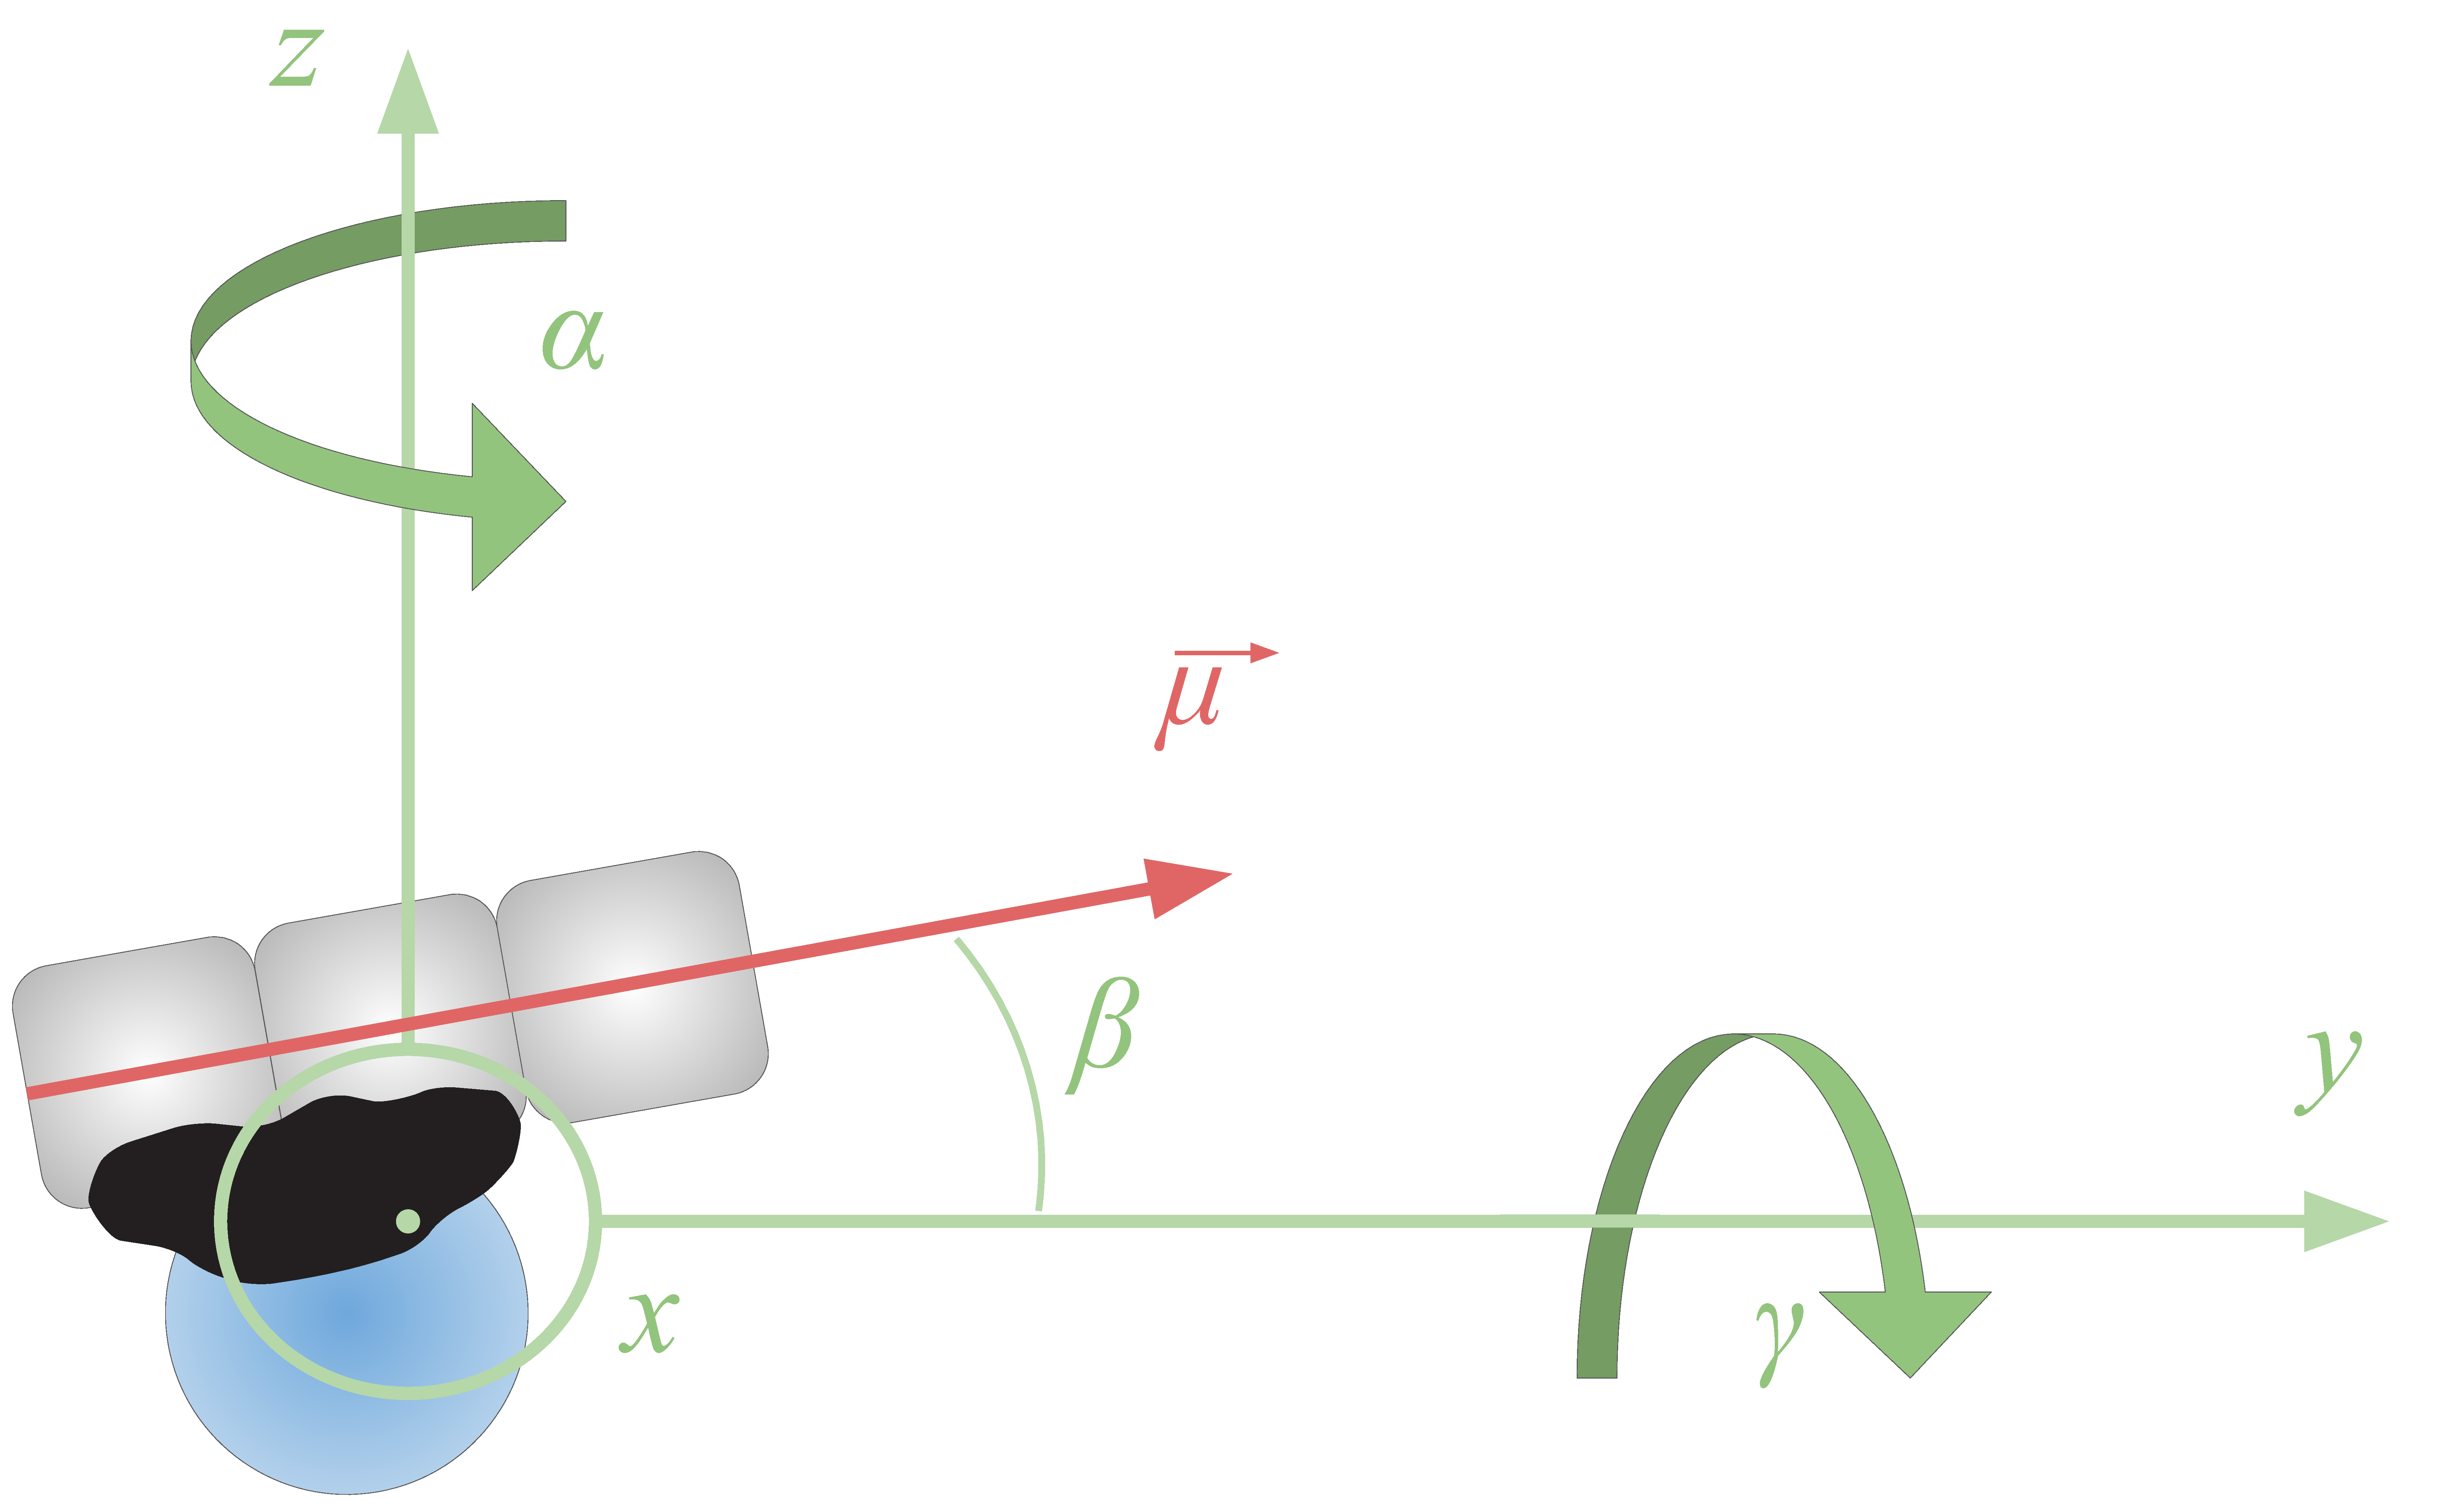
\includegraphics[width=0.63\columnwidth]{5-Appendix/Figures/Magnet_axis.pdf}
    \caption{The defined axes of the levitated magnet.}
    \label{fig:Magnet axis} 
\end{figure}

\section{B.~~Calibration of the readout circuit and energy coupling}
\makeatletter
\protected@edef\@currentlabel{B}
\label{sec:calibration}
\makeatother
\renewcommand\thefigure{\thesection B.\arabic{figure}} %To set the Fig numbering to A
\setcounter{figure}{0} 

\begin{comment}
This section is based on Supp. Mat. C in Fuchs et al.~\cite{Gravity}. 
The motion of the particle at the six resonance frequencies can be calibrated from flux to RMS motion by injecting an external current through the calibration transformer. The amount of current (or magnetic flux in the pick-up coil) injected is then directly quantified by the SQUID. The magnetic flux in the pick-up coil then exerts a force on the particle. By measuring the flux induced by the particle response, we find an absolute calibration of magnetic flux to motion. 

\begin{figure}[h]%
\centering
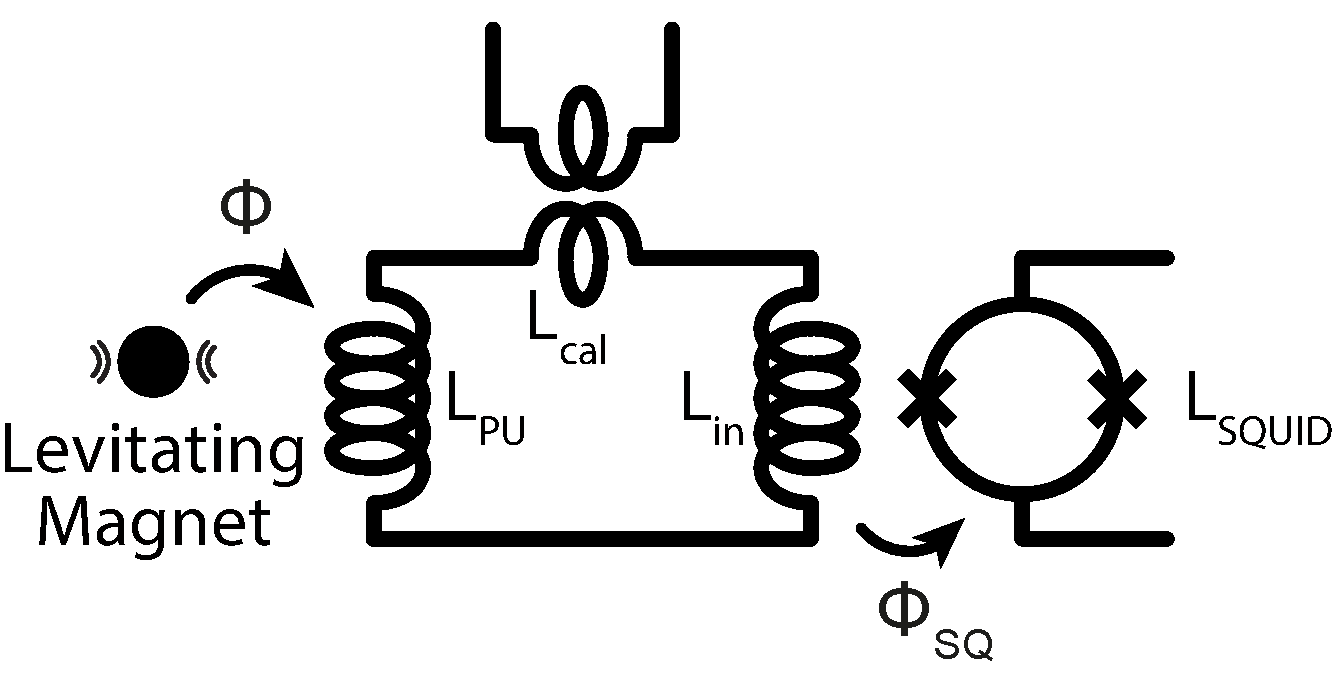
\includegraphics[width=\columnwidth]{5-Appendix/Figures/MLMP_circuit.pdf}
\caption{Schematic circuit of the single-stage readout circuit for the levitating magnet. The leviated magnet couples through a magnetic flux to the pick-up coil, with inductance $L_\text{PU}$, this flux is passed on to the SQUID via the input coil of the SQUID $L_\text{in}$ and additional flux can be added using the calibration transformer loop $L_\text{cal}$.}
\label{fig_app:readout_circuit}
\end{figure}

This calibration can be intuitively derived from the energy coupling ($\beta^2$). The energy coupling is defined as the fraction of the energies in two coupled oscillating systems, i.e. the amount of energy that couples from one system to the other. This energy coupling is similar to the quality factor of a single system, which is defined as the fraction of energy lost per cycle with respect to the total energy in the system, or equivalently, a measure for the damping of the system. Conversely, the quality factor provides a measure for the maximal energy stored in the resonator as a fraction of the input energy when driven at resonance for a time $T \gg \tau$, that is to say: the energy at which the fractional energy loss per cycle is equal to the energy put in each cycle by the resonant drive. 

For our system, with a mechanical resonator in the form of the levitating magnet, and a driving magnetic field coupled in through the calibration transformer and coupled to the magnet through the pick-up coil, we get 

\begin{equation}
    \beta^2 \equiv \frac{L_\text{total}I^2}{kx^2} 
\end{equation}

with $x$ any spatial coordinate and $L_\text{total} = L_\text{PU} + L_\text{in} + L_\text{cal}$ with the inductances as stated in Fig~\ref{fig_app:readout_circuit}. Going to the limit of infinitesimal displacement, and using $k =m\omega^2$, we obtain

\begin{equation}
    \beta^2 = \frac{\left(\frac{d\Phi}{dx}\right)^2}{L_\text{total}\cdot m\omega^2}
\end{equation}

from which it is evident that the energy coupling can be used to determine the absolute motion of the magnet from the flux measured in the SQUID.

To measure $\beta^2$, we further consider the motion of the resonator as a simple resonantly driven harmonic oscillator, with the \emph{Ansatz} $x(t) = A(t)e^{i\omega t};\ A(t) = \frac{F}{2 m \omega}\cdot t$, from which we obtain a driving force

\begin{equation}
    F_\text{driving} \left(= 2 m \zeta \omega_0 \frac{dx}{dt} = \gamma_\text{m} v \right)= \gamma_\text{m} \omega x .
\end{equation}

The quality factor ($Q_\text{drive}$) is equivalently defined as $Q_\text{drive} = \frac{1}{2\zeta}$, thus $\gamma_\text{m} = \frac{m\omega}{Q_\text{drive}}$.
In our calibration procedure, we inject a flux through the calibration transformer. This flux then results in a current through the detection circuit. This current is detected as a flux by the SQUID, with known $\frac{dI}{d\phi}$ calibration from the SQUID parameters. We refer to this current as the the crosstalk current $I_\text{crosstalk}$. This current also leads to a flux through the pick-up coil, which gives rise to a magnetic force on the particle of the form $F_\text{drive}=\alpha \cdot I_\text{crosstalk}$. Here, $\alpha$ is a coupling constant of units $\si{[N/A]}$ that contains a geometrical factor determined by both the relative positioning of the particle with respect to the pick-up coil, and the physical sizes of this coil and particle. As the particle is driven, the motion of the particle will in turn induce a current in the detection circuit. This induced current has the form $I_\text{induced}=\delta \cdot x$ where $\delta$ is a coupling constant with units $\si{[A/m]}$, which is by symmetry effected through the pick-up coil-particle geometry in the same way that $\alpha$ is.\\
Combining these results, and noting that for the steady state solution the driving force must be equal to the damping force

\begin{equation}
    \frac{I_\text{induced}}{I_\text{crosstalk}} =
    \frac{\delta\cdot x}{F_\text{drive}/\alpha} =
    \frac{\delta \cdot \alpha\cdot x}{\gamma_\text{m} \cdot \omega \cdot x} =
    Q \frac{\alpha\cdot\delta}{m\omega^2} = 
    Q \frac{\alpha\cdot\delta}{k} .
    \label{eq:I/I_1}
\end{equation}

Since some of our decay times are rather long, in our experiments we work with a $Q_\text{eff} = \pi fT_\text{drive}$, where $T_\text{drive}$ is the time during which the drive is applied. Whilst this is not the steady state, this discrepancy is fully absorbed in our definition of $Q_\text{eff}$:

\begin{equation}
    \frac{I_\text{induced}}{I_\text{crosstalk}} =
    \frac{\delta\cdot x}{F_\text{drive}/\alpha} =
    \frac{\delta \cdot \alpha\cdot x}{\gamma_\text{eff} \cdot \omega \cdot x} =
    Q_\text{eff} \frac{\alpha\cdot\delta}{m\omega^2} = 
    Q_\text{eff} \frac{\alpha\cdot\delta}{k} .
    \label{eq:I/I_2}
\end{equation}

From this derivation, we have found that the fraction of the currents in our detection circuit contains all the coupling constants in our system. In fact, looking at the units, we find
\begin{equation}
    \frac{\alpha\cdot\delta}{k} = 
    \frac{\si{\left[\frac{N}{A}\right]}\cdot\si{\left[\frac{A}{m}\right]}}{\si{\left[\frac{N}{m}\right]}}
\end{equation}
is dimensionless.

Furthermore, for small displacements in $x$, the flux change through the pick-up coil can be treated as linear. The resultant current in the detection circuit must then be $I_\text{induced} = \frac{d\Phi}{dx}\cdot x \cdot \frac{1}{L_\text{total}}$ or $\delta = \frac{d\Phi}{dx}\cdot \frac{1}{L_\text{total}} \hat{=} \si{\left[\frac{A}{m}\right]}$.

As noted before, $\delta$ contains the same geometric scaling as $\alpha$. From the symmetry, we recognise that $\alpha = \frac{d\Phi}{dx}$ ($\left[\text{Wb/m}\right]= \left[\text{N/A}\right]$). Combining these results, we find

\begin{equation}
    \frac{\alpha\cdot\delta}{k} = \frac{\left(\frac{d\Phi}{dx}\right)^2}{L_\text{total}\cdot m\omega^2} = \beta^2
\end{equation}

This final result gives us a procedure of how to measure $\beta^2$, or, conversely, the proportionality constant $\frac{d\Phi}{dx}$ that equates our measured flux to an absolute motion. The calibration measure is then found from 

\begin{equation}
    \frac{d\Phi}{dx} = \sqrt{L_\text{total}\cdot m\omega^2\cdot \beta^2} = \sqrt{L_\text{total}\cdot m\omega^2\cdot \frac{I_\text{induced}}{Q_\text{eff} \cdot I_\text{crosstalk}}}
\end{equation}

Noting that both $I_\text{induced}$ and $I_\text{crosstalk}$ are converted equally by the SQUID, the measured voltage can be inserted for the current through the detection circuit, which provides our sensitivity as 

\begin{equation}
    \frac{d\Phi}{dx} = \sqrt{L_\text{total}\cdot m\omega^2\cdot \frac{\Delta V_\text{drive}}{Q_\text{eff} \cdot V_\text{crosstalk}}}
\end{equation}

Here $\Phi$ is the flux through the pick-up coil. Since we detect this using the SQUID, we need to convert this value to the flux through the SQUID, which is done by dividing by the total inductance of the circuit and multiplying by the mutual inductance of the SQUID input loop and the SQUID loop ($M_\text{in,SQ}$). As a final step, this value can be related directly to the voltage measures made by taking the SQUID gain value as measured (${dV}/{d\Phi_\text{SQ}}$).  

The values for the inductances in $L_\text{total} = L_\text{PU}+L_\text{TP}+L_\text{in}+L_\text{cal}$ are: $L_\text{PU} = \SI{6.7e{-7}}{H}$ the inductance of the pick-up loop, $L_\text{TP} = \SI{1e{-7}}{H}$ the estimated inductance of the \SI{10}{cm} superconducting twisted-pair connecting the SQUID input to the pick-up coil, $L_\text{in} = \SI{1.8e{-6}}{H}$ the inductance of the input coil of the two-stage SQUID device, and $L_\text{cal} = \SI{2e{-9}}{H}$ the estimated inductance of the small calibration transformer coil. For the mutual inductance, the SQUID is calibrated to a value of $M_\text{in,SQ}^{-1} = \SI{0.5}{\micro A/\Phi_0}$. The SQUID voltage gain is measured as $dV/d\Phi_0 = \SI{0.43}{V/\Phi_0}$. These values, combined with measures of these ring-up's, gives us a value of $\frac{dV}{dx} = \SI{4.7}{{\frac{V}{\micro m}}}$ for mode 3 and $\frac{dV}{dx} = \SI{3.0}{{\frac{V}{\micro m}}}$ for mode 4, with a relative error of 8.5\%, which is dominated by the error in the mass.
\end{comment}

To calibrate the motion of the levitating magnet the method explained in Supp. Mat. C in Fuchs et al.~\cite{Gravity} is used. The main result of this derivation is equation S12 in this publication, giving the relationship between the measured voltage in the SQUID based measurement and the motional amplitude of the magnet, reading

\begin{equation}
    \frac{dV}{dx} = 
    \frac{dV}{d\Phi_\text{SQ}}\cdot\frac{d\Phi_\text{SQ}}{dI}\cdot\frac{dI}{d\Phi}\cdot\frac{d\Phi}{dx} =
    \frac{dV}{d\Phi_\text{SQ}} \cdot M_\text{in,SQ} \cdot \frac{1}{L_\text{total}}\cdot \frac{d\Phi}{dx}.
\end{equation}

Calculating these values for the two cooled modes gives us $\frac{dV}{dx} = \SI{4.7}{{\frac{V}{\micro m}}}$ for mode 3 and $\frac{dV}{dx} = \SI{3.0}{{\frac{V}{\micro m}}}$ for mode 4, with a relative error of 8.5\%, which is dominated by the error in the mass.

For a rotational mode the same method can be applied, and a value in units of \SI{}{[V/rad]} can be derived. To calculate a mode temperature this would result in a 
%in an integral over the angle, 
time average over the angle squared $ \left< \frac{1}{2} \kappa \theta^2 \right>_t$ in analogy to $ \left< \frac{1}{2} k x^2 \right>_t$, where $\kappa$ is the rotational stiffness, which calculates the energy in this rotational mode. If such a rotational mode is treated as a translational mode by accident and the mode temperature is calculated, the same result would be obtained as in the treatment of a rotational mode. 

%By means of conservation of energy the same energy is calculated in both cases and therefore the same mode temperature is obtained.



\begin{comment}
DU wil dit nog graag hebben voor later
\DU{wat doen we met de onzekerheid?}
\DU{Ik zou zeggen:\\
\begin{align}
    \frac{dV}{d\Phi_\text{SQ}} &\sim 1\% \\
    M_\text{in,SQ} &\sim 1\% \\
    L_\text{total} &\sim 2\% \\
    m &\sim 10\% \\
    \omega &\sim 1\% \\
    \Delta V_\text{drive} &\sim 1\% \\
    V_\text{crosstalk} &\sim 1\% \\
    Q_\text{eff} &\sim 5\% \\
\end{align}
Dan kom je uit op: 8.5\% waarbij de massa erg dominant is, als je die naar 5\% zet krijg je 5.9\% eruit, JWL: hebben we gekeken naar upper/lower bound, ik zou zeggen dat we eerder overschatten dan onderschatten, maar misschien zit ik mis
%https://www.wolframalpha.com/input?i=sqrt%280.01%5E2+%2B+0.01%5E2+%2B+0.02%5E2+%2B+1%2F2*%280.02%5E2%2B0.10%5E2%2B2*0.01%5E2+%2B+0.01%5E2+%2B+0.01%5E2%2B0.05%5E2%29%29
}
\DU{we doen 8.5\%}\\
\end{comment}

\section{C.~~Mode mixing due to nonlinearities}
\makeatletter
\protected@edef\@currentlabel{C}
\label{sec:mode mixing}
\makeatother
\renewcommand\thefigure{\thesection C.\arabic{figure}} %To set the Fig numbering to B
\setcounter{figure}{0} 

The signal detected by the SQUID contains not only the six modes related to the six degrees of motion of the magnetic particle (three librations and three translations). It also contains other vibrational movement of the setup. Modes of the mass spring system are most prominent in the \SIrange{0.5}{15}{Hz} range, see Fig.~\ref{fig:spectrum_mass_spring}. 

\begin{figure}[h]
    \centering
    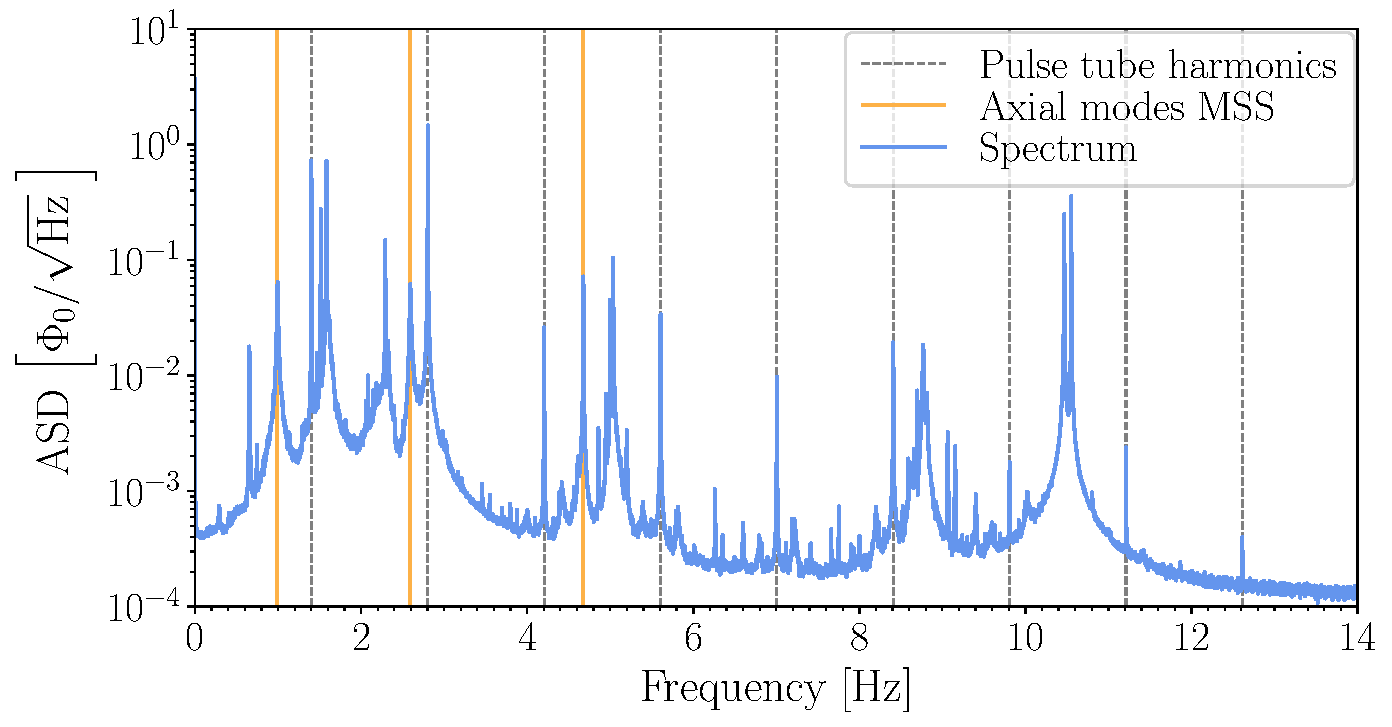
\includegraphics[width=\columnwidth]{5-Appendix/Figures/paper_spectrum_mass_spring_small_good2.pdf}
    \caption{Typical ASD of the resonances of the mass spring system as measured by the SQUID that measures the relative motion between the levitated magnet and pick-up coil. Multiples of the pulse tube frequency (\SI{1.401}{Hz}) are indicated with the vertical dashed lines. The axial modes of the mass spring system (MSS) as simulated are indicated with the vertical lines.}
    \label{fig:spectrum_mass_spring} 
\end{figure}

Many of these peaks in the spectrum can be attributed to vibrations caused by either the cooling equipment or the resonances of the vibration isolation system. Using a finite element model, we can link certain frequencies to modes of the mass spring system (MSS).

In Fig.~\ref{fig:spectrum_attenuation}, a finite element simulation transfer function is plotted of both the lateral and axial motion of the MSS to the experiment. To generate these plots, a simplified model is solved using a finite element method. Here, the three masses are simulated as perfect cylinders, and the helical springs are idealized as perfectly elastic snare springs, and their spring constants are physically measured at room temperature and extrapolated to cryogenic temperatures.

We observe that the simulated axial modes (vertical motion) of the MSS align directly with some of the measured peaks in the spectrum. Other peaks in the spectrum can be explained by the lateral and rotational movement of the mass spring system. Comparing between the simulation and the measurements, the values do not all coincide, but some are shifted with the highest mode at \SI{10.5}{Hz}.

\begin{figure}[h]
    \centering
    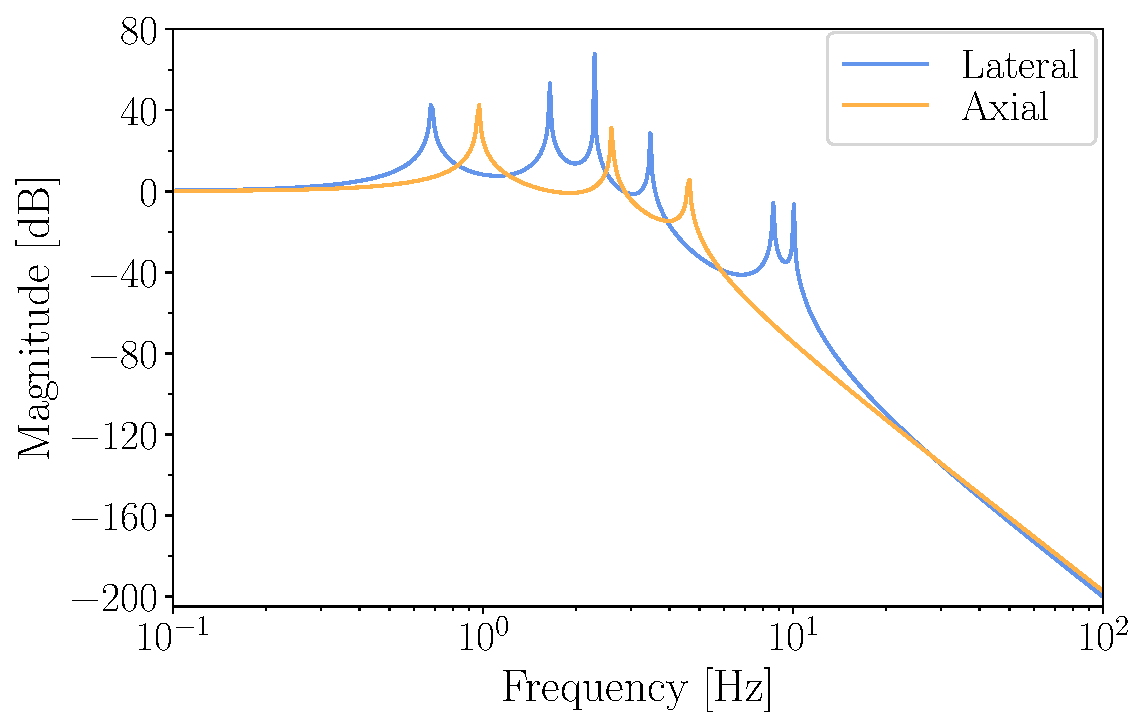
\includegraphics[width=\columnwidth]{5-Appendix/Figures/paper_spectrum_attenuation_log10.pdf}
    \caption{Bode magnitude plot of the attenuation of both the lateral and axial motion of the mass spring system (MSS), simulated with a finite element model.}
    \label{fig:spectrum_attenuation}
\end{figure}

During the experiment, we also observe peaks in the spectrum at frequencies that are the sum or difference of two peaks elsewhere in the spectrum. The most clear example can be seen in Fig.~\ref{fig:upconversion_mode_3} at \SI{51.5}{Hz}, where the peak displaced by \SI{0.92}{Hz} to the left of the resonance at a frequency of \SI{49.67}{Hz} is clearly reflected in the resonance of the magnet to \SI{51.51}{Hz}. This upconverted noise is cooled simultaneously with the resonance peak, meaning that the noise is coupled in through the motion of the magnet, the amplitude of the mode decreases with increasing gain and also the \SI{51.5}{Hz} noise decreases with increasing gain. We attribute the noise peak at \SI{49.67}{Hz} to a snare mode of the bottom spring of the vibration isolation system that we find in some finite element simulations. This mixing occurs because of the non-linearity of the trapping potential, which arises from the non-linear magnetic potential.

\begin{figure}[h]
    \centering
    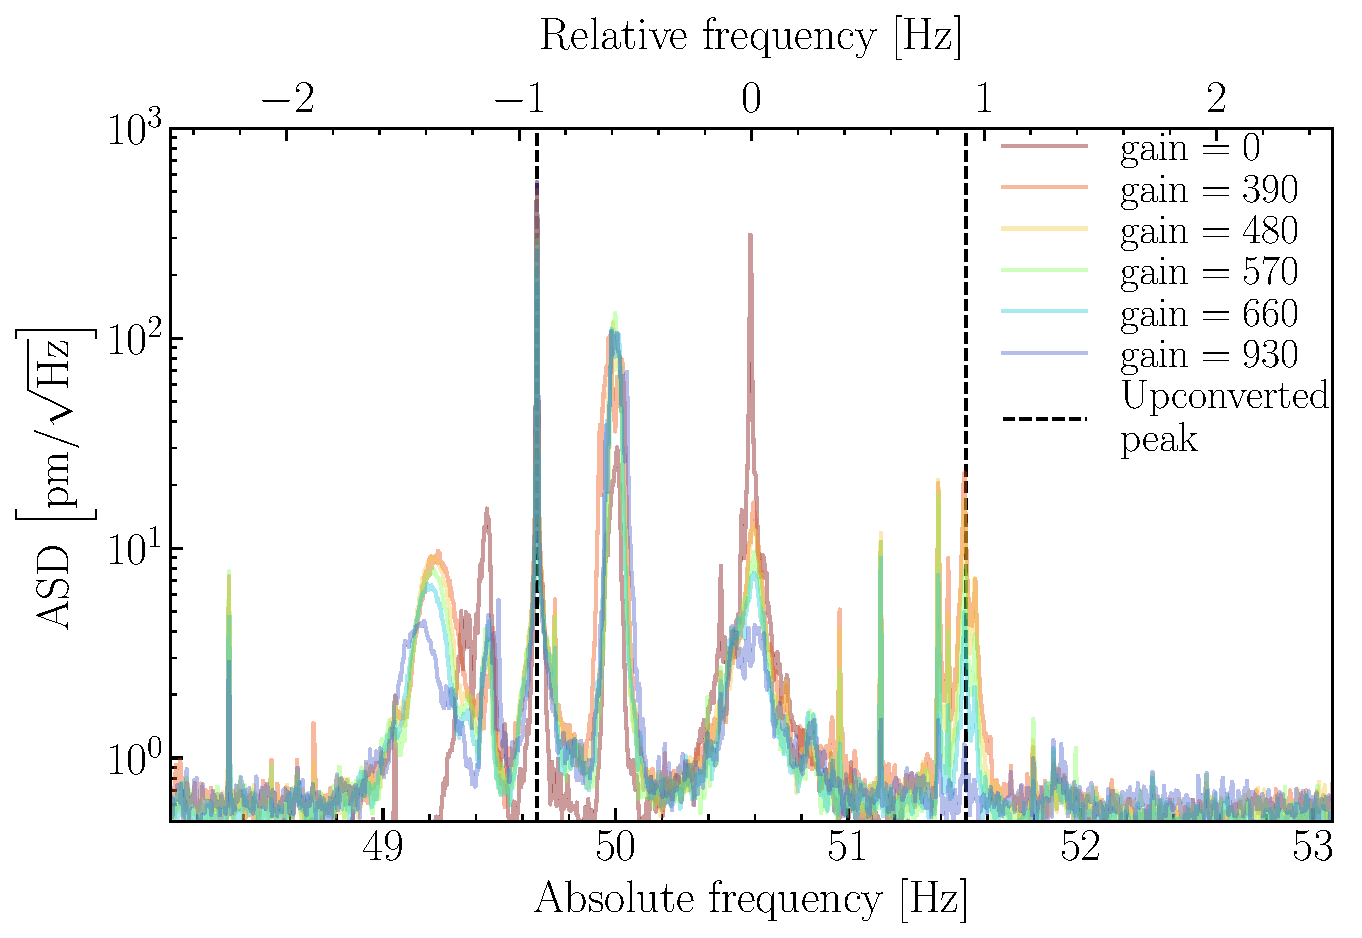
\includegraphics[width=\columnwidth]{5-Appendix/Figures/paper_appendix_upconversion_mode_3.pdf}
    \caption{The spectrum around mode 3, where upconversion can be seen at for example \SI{51.5}{Hz}.}
    \label{fig:upconversion_mode_3} 
\end{figure}

Please note that when we perform mode cooling and bring the particle motion of a translational mode down to a few picometers, the amplitude of the relative motion between the magnet and the trap at lower frequencies (\SIrange{0.5}{15}{Hz}) remains unchanged, and can be more than four orders of magnitude in amplitude larger as is visible in Fig~\ref{fig:spectrum}. For the \SI{50.6}{Hz} mode, mechanical vibrations of the compressor and circulation pumps of the dilution refrigerator (which are often slightly below \SI{50}{Hz}) mix with the mechanical modes of the vibration isolation system. We cannot account for all the peaks we see, but we attribute this to upconversion of several peaks mixing together to work against us. Also we cannot exclude that \SI{50}{Hz} electrical noise interferes with mechanical vibrations. Therefore we conclude that to improve the feedback cooling further we will need to also perform linear feedback cooling on the modes of the vibration isolation system.




%In Fig.~\ref{fig:upconversion_mode_3} and Fig.~\ref{fig:upconversion_mode_4} we show the upconversion around the two cooled modes. The most clear example can be seen in Fig.~\ref{fig:upconversion_mode_3} at \SI{51.5}{Hz}, this upconverted noise is cooled simultaneously with the resonance peak. Meaning that the noise is coupled in through the motion of the magnet, the amplitude of the mode decreases with increasing gain and also the \SI{51.5}{Hz} noise decreases with increasing gain.



%\end{comment}
\end{document}